\documentclass[]{standalone}
\usepackage[T1]{fontenc}
\usepackage{tikz}
\usepackage{amsmath, amsfonts}
\usepackage{xintexpr}
\usepackage{xparse}
\usepackage{comment}
\usepackage{ifthen}
\usetikzlibrary{arrows, shapes.geometric, calc, positioning, decorations.pathreplacing, patterns.meta}

\makeatletter
\def\input@path{{./includes/}{./includes/ut/diags/}}
\makeatother

\definecolor{malachite}{rgb}{0.04, 0.85, 0.32}
\definecolor{mikadoyellow}{rgb}{1.0, 0.77, 0.05}
\definecolor{fluorescentpink}{rgb}{1.0, 0.08, 0.58}

\begin{document}%
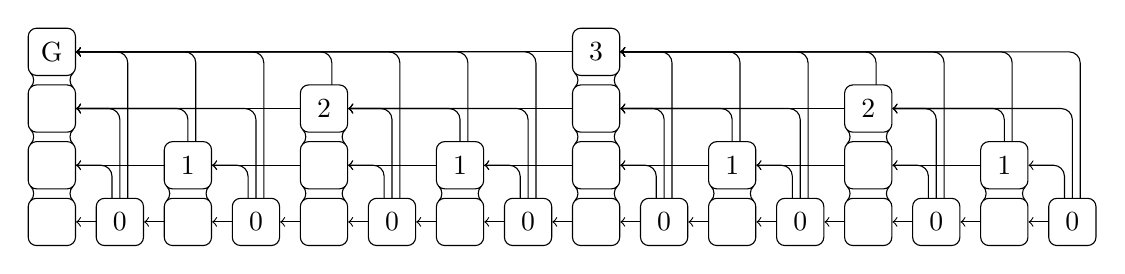
\begin{tikzpicture}[]
    \def\scale{0.6cm}
    \edef\blockWH{\scale}
    \def\spacingMult{1.2}
    \edef\sx{1.2*\spacingMult*\scale}
    \edef\sy{\spacingMult*\scale}

    \tikzstyle{block} = [draw, rounded corners=3pt, align=center, minimum width=\blockWH, minimum height=\blockWH]

    \def\bheights{{3,0,1,0,2,0,1,0,3,0,1,0,2,0,1,0}}
    \xdef\maxMu{3}
    \pgfmathtruncatemacro{\maxMuPOne}{\maxMu + 1}

    \foreach \h in {0,...,15} {
        \pgfmathsetmacro{\blockMu}{\bheights[\h]}
        \foreach \m in {0,...,\blockMu} {
            \xdef\blockLabel{}
            \ifnum \m=\blockMu
                \xdef\blockLabel{\blockMu}
                \ifnum \h=0
                    \xdef\blockLabel{G}
                \fi
            \fi
            \node (n-\h-\m) [block] at (\h*\sx, \m*\sy) {\blockLabel};

            % draw lines to lower blocks
            \ifnum 0<\m
                \pgfmathtruncatemacro{\lastM}{\m - 1}
                % \draw [double distance=11pt] (n-\h-\m) -- (n-\h-\lastM);
                %shorten >= -3pt, shorten <= -3pt, smooth
                \draw []
                    % ($(n-\h-\m.south west)!.5!(n-\h-\lastM.north west)$)
                    ($(n-\h-\m.south west) + (1.1pt, 1.1pt)$)
                    arc (45:-45:3.65pt)
                    ($(n-\h-\m.south east) + (-1.1pt, 1.1pt)$)
                    arc (-45:45:-3.65pt);
                    % ($(n-\h-\m.south west) + (2pt, -0.2pt)$)
                    % -- ($(n-\h-\m.south west)!.5!(n-\h-\lastM.north west) + (3pt, 0)$)
                    % -- ($(n-\h-\lastM.north west) + (2pt, 1pt)$);
            \fi

            % no arrows for h=0
            \ifnum 0<\h
                % draw arrows to past blocks
                \pgfmathtruncatemacro{\prevBlockAtMu}{\h - 2^\m}
                \draw [->] (n-\h-\m) -- (n-\prevBlockAtMu-\m);
                % if we're the top square in this column, draw arrows to higher mu blocks
                \ifnum \m=\blockMu
                    \pgfmathtruncatemacro{\nextMu}{\blockMu + 1}
                    \foreach \pm in {\nextMu,...,\maxMu} {
                        \ifnum \nextMu<\maxMuPOne
                            \pgfmathtruncatemacro{\prevHiMuX}{\h - mod(\h, 2^\pm)}
                            \pgfmathsetmacro{\arrowXOffs}{\pm}
                            \draw [->, rounded corners] ($(n-\h-\m.north) + (\pm mm - 2 mm, -.2pt)$) |- (n-\prevHiMuX-\pm);
                        \fi
                    }
                \fi
            \fi
        }
    }
\end{tikzpicture}%
\end{document}
